\chapter{Script de comparaison}

N'ayant pas de notions de programmation orientée objet\, \footnote{Ce qui sera
enseignée en deuxième année.} je n'ai pas pu rejoindre les développeurs de
l'entreprise dans l'application qu'ils développaient, cela dit on m'a confié
une tâche annexe qui est la comparaison des bases de données. Le schéma
\ref{bdd} en page \pageref{bdd} nous en illustre une structure basique.

\begin{figure}
\begin{center}
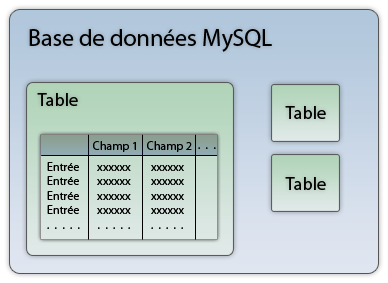
\includegraphics[scale=0.5]{images/bdd.png}
\end{center}
\caption{Un schéma de base de données simple.}
\label{bdd}
\end{figure}

Le besoin premier de ce script est de consulter les différences qui existent
entre une base de référence est une base à mettre à jour. Dans le cas de
l'entreprise, il permettrait un suivi des mises à jour des applications
fournies au client et pour moi, m'initier à la programmation orientée objet\,
\footnote{La programmation orientée objet est un paradigme de programmation qui
consiste à utiliser des objets ; un objet représente un concept, une idée ou
toute entité du monde physique, comme une voiture, une personne ou encore une
page d'un livre.} dès le premier stage.

\section{Le départ}

À l'aide d'un cours sur internet, j'ai commencé à créer ma première classe.
Cette classe après instanciation représenterait l'objet \og base de données
\fg{} sous forme de tableau. L'image \ref{obj} qui ce trouve en page
\pageref{obj} est plus parlante.

\begin{figure}
\begin{center}
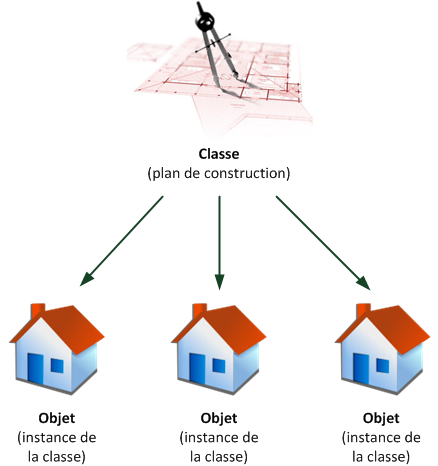
\includegraphics[scale=0.5]{images/objet.png}
\end{center}
\caption{Un plan à partir duquel on crée des objets.}
\label{obj}
\end{figure}

Passer de la programmation fonctionnelle\, \footnote{La programmation
fonctionnelle est un paradigme de programmation qui repose sur l'utilisation
majoritaire des fonctions et procédures.} à l'objet fut vraiment difficile. Me
rendant compte que je bloquais énormément, je fis des recherches sur internet
pour trouver un programme équivalent sur lequel je me suis appuyé pour
commencer. M.\bsc{Dubourg} m'a mis sur la voie en me disant d'utiliser des
classes et des méthodes toutes prêtes de l'entreprise ce qui me fit gagner
beaucoup de temps, car je savais pas comment transcrire une structure de base
de données en objet.

Pour utiliser les sources de la société, j'ai dû mettre en place un répertoire
de travail et récupérer les sources via leur ancien gestionnaire de version de
code source. Ceci étant fait il s'agissait maintenant de réussir à faire
fonctionner le site web principal en local sur ma machine. Comme mon logiciel
MAMP\, \footnote{\emph{Macintosh Apache MySQL PHP.} est une combinaison de
logiciel.} m'affichait plein d'erreurs, j'ai décidé d'installer manuellement
chacun des logiciels présents dans celui-ci. Même après cette manipulation le
problème n'avait pas disparu, mon tuteur de stage m'est venu en aide après de
longues heures à chercher en vain. Le problème était tout d'abord au niveau de
la configuration de PHP, qui affichait tous les avertissements de manière trop
stricte, ce qui entravait le lancement de la page principale. Il était aussi au
niveau du cache de mon navigateur. En effet, j'ai du vider celui-ci pour faire
enfin apparaitre le site proprement. De nombreuses heures de recherche juste à
cause d'un cache internet non vidé fut extrêmement frustrant \ldots{}

\section{Comparaison des tables}

Il a fallu dans un premier temps que je recherche comment extraire le nom d'une
base ainsi que le nom de ses tables. La réponse à cette question est dans la
documentation de MySQL. Une base de données est fournit à l'installation et
s'appelle \og information schéma \fg{} . En résumé, c'est une base de données
qui contient toutes les autres.

Ensuite, j'ai transformé le programme procédural sur plusieurs semaines en
objet, le fait de passer par cette étape intermédiaire m'a permis d'abord de
résoudre le problème algorithmiquement, puis de me consacrer sur la façon de
l'écrire.

La requête récupérant les données utiles, j'ai dû concevoir un algorithme
capable de comparer les deux tableaux d'objets par rapport à leurs noms :
\begin{itemize}
    \item Si la base de données de référence a une table qui n'est pas dans
    la base de données à mettre à jour, on l'ajoute ;
    \item Si la base de données à mettre à jour contient une table qui n'est
    pas dans la base de données de référence, on l'enlève ;
    \item Si les tables comparées sont toutes les deux dans les bases de
    données, on compare l'intérieur des tables.
\end{itemize}

J'ai dû revoir mon algorithme plusieurs fois, car la fonction de comparaison de
chaine de caractère \texttt{strnatcmp} compare les mots comme un humain le
ferait, alors que mySQL trie les tables de manière binaire grâce aux codes
ASCII\, \footnote{\emph{American Standard Code for Information Interchange.} ou
\og Code américain normalisé pour l'échange d'information \fg{} est la norme de
codage de caractères en informatique la plus connue, la plus ancienne et la
plus largement compatible.} des caractères ce qui faisait que la première
fonction donnait des résultats erronés comme le montre le tableau \ref{tab}.

\begin{table}
\begin{center}
\begin{tabular}{|c|c|}
\hline
\textbf{Tri de chaînes standard} & \textbf{Tri de chaînes ordre naturel} \\
\hline
[0] = img1.png & [0] = img1.png \\
\hline
[1] = img10.png & [1] = img2.png \\
\hline
[2] = img12.png & [2] = img10.png \\
\hline
[3] = img2.png & [3] = img12.png \\
\hline
\end{tabular}
\caption{La différence entre les tris de chaînes.}
\label{tab}
\end{center}
\end{table}

\section{Comparaison des champs}

J'étais dans la situation des tables ayant les mêmes noms, il fallait que je
compare le contenu à partir du nom des champs. Il ne m'a pas fallut longtemps
pour comprendre que l'algorithme était exactement le même, le plus dur étant de
savoir comment j'allais faire pour ne pas me répéter, ce qui a bloqué
énormément mon avancé pour pas grand-chose. M.\bsc{Dubourg} constatant que je
stagnais, m'a conseillé de faire comme j'avais appris plutôt que d'essayer de
faire de la POO\, \footnote{\emph{Programmation Orientée Objet.}}.  Une fois le
script fonctionnel, qui était cependant mal optimisé et peu lisible, mon tuteur
me guida avec des explications poussées sur la marche à suivre. De fil en
aiguille le code source passa d'environ trois-cent cinquante lignes à cent
cinquante.

Ensuite, je devais comparer le contenu des champs des tables lorsque les champs
parcourus avait le même nom. Je comparais tout simplement le contenu des champs
pour connaitre l'issue finale, à savoir que je ne pouvais pas décider si les
tables étaient similaire sans avoir balayé tous les champs et toutes les
caractéristiques de ceux-ci.

\section{Affichage du résultat}

Après tout ceci fini et optimisé, j'implémente une nouvelle fonctionnalité qui
permettrait d'afficher un texte lisible qui énonce les différences des deux
bases de données. En fonction des résultats obtenus, je génère des balises HTML\,
\footnote{L’ \emph{Hypertext Markup Language} est un langage de balisage conçu
pour représenter les pages web.} et du texte pour que cela soit compréhensible
à l'utilisateur. Ceci étant fait assez rapidement je suis passé à la génération
des requêtes SQL\, \footnote{\emph{Structured Query Language} est un langage
informatique normalisé qui sert à effectuer des opérations sur des bases de
données.} permettant de mettre à jour la base obsolète depuis la base de
référence. C'est à ce stade que j'ai constaté que je ne pourrais pas prendre en
compte les clés étrangères dans mon code à moins de revoir totalement tout le
script. M.\bsc{Dubourg} m'a rassuré sur le fait que l'entreprise n'utilisait pas
le type de base de données myISAM\, \footnote{L'organisation séquentielle
indexée, ou \emph{Indexed Sequential Access Method} en anglais, est un mode
d'organisation des fichiers dans les bases de données.} et que donc aucune de
leurs tables comportait de clé étrangère, cependant les clés primaires
concaténées restent problématiques, car pas imaginer pendant la conception. Nous
avons décidé que la création de ce genre de cas se fera à la main pour ne pas
repartir de zéro.

Après avoir analysé mes méthodes de génération de phrases lisibles et de
requêtes SQL, M.\bsc{Dubourg} m'a présenté un outil nommé \og Smarty \fg{} qui
permet de dissocier la partie traitement de la partie affichage, car il est
vrai que mes méthodes étaient vraiment très sales. Pour résumer, j'écrivais des
chaînes de caractères dans une seule variable en écrivant les noms des tables
ou des champs, en concaténant le tout avec des balises HTML de saut de ligne un
peu n'importe où. J'ai dû parcourir la documentation de Smarty pour comprendre
son fonctionnement, il s'avère que la syntaxe est très particulière mais très
efficace. J'ai terminé par faire de l'agencement sur ma page pour que chaque
ligne lisible par un néophyte soit en face de la ligne traduite en SQL dans un
tableau à deux colonnes.

\clearpage
